% -----------------------------------------------
% Template for ISMIR Papers
% 2025 version, based on previous ISMIR templates

% Requirements :
% * 6+n page length maximum
% * 10MB maximum file size
% * Copyright note must appear in the bottom left corner of first page
% * Clearer statement about citing own work in anonymized submission
% (see conference website for additional details)
% -----------------------------------------------

\documentclass{article}
\usepackage[T1]{fontenc}
\usepackage[utf8]{inputenc}
\usepackage{ismir} % Remove the "submission" option for camera-ready version
\usepackage{amsmath,cite,url}
\usepackage{graphicx}
\usepackage{color}

% Title. Please use IEEE-compliant title case when specifying the title here,
% as it has implications for the copyright notice
% ------
\title{Project Specification for CSC 475 \conferenceyear: TransVox}

% Note: Please do NOT use \thanks or a \footnote in any of the author markup

% Single address
% To use with only one author or several with the same address
% ---------------
%\oneauthor
 %{Isaiah Doyle, Aileen Klassen, Elijah Larmer}

  %{University of Victoria\\\texttt{anonymous@ismir.net}}


% Two addresses
% --------------
%\twoauthors
%   {First author} {School \\ Department}
%   {Second author} {Company \\ Address}

%Three addresses
%--------------
\author{
   \textbf{Isaiah Doyle}\\ {University of Victoria \\\texttt{isaiahdoyle@uvic.ca}}
   \and
   \textbf{Aileen Klassen}\\ {University of Victoria\\\texttt{aileenklassen@uvic.ca}}
   \and
   \textbf{Elijah Larmer}\\ {University of Victoria \\\texttt{elijahlarmer@uvic.ca}}
}

% Four or more addresses
% OR alternative format for large number of co-authors
% ------------
% \multauthor
%   {First author$^1$ \hspace{1cm} Second author$^1$ \hspace{1cm} Third author$^2$}
%   {{\bf Fourth author$^3$ \hspace{1cm} Fifth author$^2$ \hspace{1cm} Sixth author$^1$}\\
%   $^1$ Department of Computer Science, University, Country\\
%   $^2$ International Laboratories, City, Country\\
%   $^3$ Company, Address\\
%   {\tt\small CorrespondenceAuthor@ismir.edu, PossibleOtherAuthor@ismir.edu}
%   }

% For the author list in the Creative Common license, please enter author names.
% Please abbreviate the first names of authors and add 'and' between the second to last and last authors.
\def\authorname{Doyle, I., Klassen, A., \& Larmer, E.}

% Optional: To use hyperref, uncomment the following.
% \usepackage[bookmarks=false,pdfauthor={\authorname},pdfsubject={\pdfsubject},hidelinks]{hyperref}
% Mind the bookmarks=false option; bookmarks are incompatible with ismir.sty.

\sloppy % please retain sloppy command for improved formatting

\begin{document}

\maketitle{}


\begin{abstract}
  The state of programs designed to support voice training are lacking with respect to timbral nuance. For trans people undergoing voice training, available applications tend to favour pitch as the primary – or in some cases sole – measure of progress. To accommodate the many parameters that factor into voice perception, we propose a tool to allow users to mimic a resynthesized version of their voice using applied timbral descriptors.
\end{abstract}


\section{Introduction}\label{sec:introduction}

This project is a component of a larger application that supports people undergoing voice training in developing their preferred vocal timbre by mimicking a synthesized version of their voice with any desired timbral modifications. Current applications \cite{DevExtras}, \cite{SeekAndNitz}, \cite{AntoniAndSpeechtools}, \cite{Alter24} have relied largely on pitch to distinguish vocal characteristics. Vocal perception is more complex than this, and as such timbral development of those undergoing voice training is paramount to users’ success \cite{HawleyAndHancock24}. Semantic timbral descriptors (e.g., breathier, huskier, higher) will be given by the user to apply to a recording of their voice, and the resulting output can be tweaked further using additional descriptors.

By using the user’s voice as the primary input source, our goal is to promote a healthy and informed way to explore the timbral possibilities of one’s voice. The long term goal is to package this into an accessible vocal coach, acting as a tool for speech pathologists and the public (e.g., trans people seeking a more feminine/masculine/neutral voice, people with speech impairments \cite{Barkmeier-Kraemer}, voice actors).

This document first outlines project goals, then tools and resources used during development. A timeline of work follows, concluding with a log of experiments and their results.


\section{Goals}\label{sec:page_size}
\begin{enumerate}
    \item Basic goals include being able to have code that can adjust and change the user's voice per their specifications. We want to include different options to re-synthesize the given audio and have it return a natural-sounding voice. This would include pitch, breathiness and other textures as mentioned previously.
    \item A step up is to include having a method that lets the user upload their audio to our program so that they can adjust their audio. This can be done using a simple HTML page where a user can upload and choose which adjustments they would like to do. Adjustments would be made in set intervals where the user would be able to choose their own levels of adjustment.
    \item A stretch goal would to be able to create a detailed and customized interface for the user to be able to interact with. This would include more specific JavaScript interactive objects such as dials, fine tune levels and options. Design would be initially done in Figma and then would be translated to HTML/CSS/JS format to create a memorable, interactive interface.
\end{enumerate}


\section{Methodology}

Python is the driving coding language for this project. FreeVC \cite{Li22} has proven to be a wealth of information regarding voice cloning, featuring the implementation of libraries like pytorch \cite{PyTorch} and Librosa \cite{Librosa} to support speech analysis and synthesis using a fine-tuned checkpoint of Microsoft's WavLM model \cite{WavLM}. FreeVC first extracts a generalized timbre (i.e., mel-frequency cepstral coefficients) cepstrogram from a sample of a 'target' voice, then uses WavLM to extract the content (i.e., words spoken) from a sample of a 'source' voice. A custom transformer is then used to infer a .wav file containing the content from the source speaker using the timbre of the target speaker.

We have used FreeVC as a guideline for our own implementation of speech resynthesis, and we use similar libraries to train a separate model to allow timbral adjustments to be made to the output by intercepting and modifying the MFCC cepstrogram before resynthesis.


\section{Timeline}\label{sec:page_size}

There was a significant learning curve for all members while implementing this project, so details were subject to change throughout the term. The following timeline represents the work undergone as of April 16, 2025 including all changes since the previous timeline from March 18:

\begin{enumerate}
  \item Before commencing the project, it was important that all members are on the same page and agree to and understand the project details and distribution of work. Amendments would be made to this timeline as research progresses and implementation details are decided on.
  \item There are two major components to the project - the first being effectively cloning a vocal sample. We eventually decided on using FreeVC as a primary reference. We anticipated having a working model by early March, but the following dates are when related work was completed:
    \begin{itemize}
      \item Mar. 10: discovered FreeVC (Isaiah)
      \item Mar. 13: got FreeVC working, effectively cloning a speech sample via resynthesis (Isaiah)
      \item Mar. 18: developed a proof of concept for adjustment of timbral quality by manual intervention (Isaiah)
    \end{itemize}
  \item The second component involves the development of a trained model to modify vocal timbre. This includes deciding on the number of descriptors we want to use (if a finite number), and labelling a dataset of speech samples with those descriptors. We had first considered using effects that mimic timbral changes (e.g., breathiness by linear predictive coding \cite{Nordstrom08}) to generate this dataset, but decided on manual rating to support more descriptors. This was anticipated to be completed by mid-March.
    \begin{itemize}
      \item Mar. 8: determined which descriptors to use (Aileen, Elijah, Isaiah)
      \item Mar. 15: implemented a pitch shifting effect (Elijah)
      \item Mar. 17: implemented an effect to adjust perceived 'roughness' of a voice (Aileen)
    \end{itemize}
  \item What remained was then to complete a labelled dataset to train an MFCC classification model with, and use it to infer the adjustments to be made to an arbitrary MFCC cepstrogram (representing a voice) in order to mold it into a desired timbre.
    \begin{itemize}
      \item Apr. 1: create a program for manually labelling the dataset (Aileen)
      \item Apr. 12: complete a labelled dataset mapping MFCC cepstrograms to timbres (Aileen, Elijah, Isaiah)
      \item Apr. 12: train classifiers on said dataset to model trends  (Elijah)
      \item Apr. 15: complete timbral manipulation using trends on input MFCC cepstrograms (Isaiah)
      \item Apr. 16: final adjustments (Aileen, Elijah, Isaiah)
    \end{itemize}
\end{enumerate}

There were difficulties in modelling timbral adjustment due to a lack of research currently, so there were significant setbacks in the initial timelines. We spent more time working with creating a dataset to train a model and analysing MFCC's. Though we have been behind, we are happy with the progress that we have been able to make within this project.

\section{Experiments}\label{sec:page_size}

We began by exploring a number of potential methods in trying to get past the initial phase of resynthesizing a recording of human speech. Going in we knew it would be critical, due to the intent behind the project, for the output to be realistic (i.e., imitable by a human within reason), and to have manual control over the timbre of the output. The first method we explored was the application of linear predictive coding, as we were all familiar with historical examples of using LPC for vocal modifications like pitch shifting \cite{SasahireAndHashimoto95}. As we explored using LPC, it became clear that the outputted audio sounded rough and robotic, which was a deal-breaker since we required that the output sound as natural as possible.

Mel-frequency cepstral coefficients were considered early on due to their generalized, but effective, characterization of timbre, and its proven applications in speech processing \cite{Ittichaichareon12}. Although MFCCs are indeed able to extract vocal features and represent an audio file's timbral characteristics - even going as far as to be able to identify the speaker's emotion \cite{Lalithaa15} - it seemed to us that MFCCs lacked the granularity required to faithfully re-synthesize an audio sample. Unlike frequency spectra, choosing a discrete number of MFCCs to analyze results in loss of information, making it impossible to invert the operation to obtain the unchanged input. That is, using a sample's MFCCs to re-synthesize the audio results in a thin, coarse and robotic sound due to the temporal information lost in the process.

As neither LPC or MFCCs seemed to be able to retrieve the information we needed from the audio as well as provide enough information to re-create the audio, we briefly changed course toward a simpler approach. In the interest of getting a tangible proof of concept, we decided to program distinct functions for adjusting the pitch, tone, breathiness, and roughness associated with input audio. With these functions, we proposed that users would adjust a number of sliders mapping to the prominence of the aforementioned effects, thus removing the need for any kind of speech synthesis.

We were still keen on researching speech re-synthesis though, so we allocated time and effort into diving deeper. We eventually stumbled upon source code claiming to effectively re-synthesize input speech using the content from one speaker using the timbre of another. FreeVC \cite{Li22} works by first encoding speech information (i.e., the words spoken) by providing the raw 'source' waveform to a pre-trained WavLM model and bottleneck extractor. The timbre of another 'target' waveform is then extracted by computing a mel-cepstrogram, such that the content of the source waveform and mel-cepstrogram of the target waveform are used as input to a HiFi-GAN v1 vocoder \cite{Kong20} for synthesis.

The approach Li et. al \cite{Li22} employ allow for the modification of MFCC timbral information before inference, thus allowing the possiblity of timbral adjustment. This motivated us to get back on track with our original plan, pursuing the use of MFCC manipulation as a means for timbral adjustment. We spent some time tinkering with the FreeVC source code to familiarise ourselves with its inner workings and explore the timbral possibilities of this approach.

Each frame of the extracted mel-cepstrogram from the target waveform, by FreeVC's defaults, contains 80 MFCCs taken at intervals of 320 samples with a window size of 1280 samples. These are organized in a pytorch \texttt{tensor} object, which takes a form similar to a 3-dimensional numpy array, supporting the same operations for data access and modification (e.g., \texttt{tensor([[[A1, B1, ...], [A2, B2, ...], ..., [A80, B80, ...]]])} represents a mel-cepstrogram of some number of 80-coefficient mel-cepstra). Thus, we were able to manually modify the mel-cepstrogram before resynthesis to observe its effects. The following is an example of halving the magnitude of the 40 upper MFCCs (the upper half of the mel-cepstrum) for all cepstra in the extracted mel-cepstrogram:

\begin{verbatim}
mel_cepstrogram[:, 40:, :] *= 0.5
\end{verbatim}

The quality of the results were varied, which is to be expected given the brute-force nature of the experimental procedure. There was undeniably, however, considerable timbral change in the synthesized output, so we were optimistic that a more informed approach to MFCC modification will allow the program to adjust the synthesized timbre in an intuitive way.


\subsection{Dataset}

We utilized a subset of the Common Voice dataset [16] as the foundation for our analysis. Given the extensive size of the dataset, we selected 900 audio files for further processing. This involved filtering out samples that were too quiet, contained excessive background noise, or had unintelligible speech. After curating a set of high-quality and usable audio samples we completed our dataset by rating each sample on a five-point scale for breathiness (1: not at all, 5: very breathy), pitch (1: low, 5: high), smoothness (1: rough/raspy, 5: smooth/podcast-y) and tone (1: thin/nasally, 5: full/strong). This was done using a custom Python program that led each of us through the library, prompting for ratings for each sample according to the parameters above. The data was then output into a spreadsheet that was uploaded to OneDrive for syncing purposes. There were some small hiccups where the file wasn't updated correctly, but with version control we were able to recover and reinstate any lost data from syncing issues. The spreadsheet would record the ratings from each user (Aileen, Elijah, Isaiah), then record the average of all our rankings in a separate final column. There was also a feature to replay the audio clip as needed during ranking, as well as being able to save your progress and return to the same point at another time. This streamlined the labelling process, and allowed us to reasonably process a large number of files manually.

Using this labeled dataset, we developed predictive models for each vocal parameter. Initially, we employed Gaussian Naive Bayes models, using the MFCCs for each audio track as input features. MFCCs were extracted for each audio file using a custom \texttt{get\_timbre()} method in our implementation of FreeVC \cite{Li22}. Data preprocessing and model development were conducted using the pandas \cite{Pandas} and scikit-learn \cite{Sklearn} libraries. The dataset was split evenly into training and testing subsets.

The following are the performance metrics (precision, recall, and F1-score) for each attribute, evaluated on the test set using the Gaussian model (see \tabref{tab:gpitch}, \tabref{tab:gtone}, \tabref{tab:gbreath}, and \tabref{tab:gsmooth}).

\begin{table}
\begin{verbatim}
  precision  recall  f1-score  support

1     0.12     0.44      0.19       32
2     0.70     0.22      0.33      208
3     0.09     0.39      0.15       23
4     0.26     0.21      0.23       63
5     0.20     0.33      0.25        3

accuracy                 0.25      329
\end{verbatim}
\caption{GNB classification report for pitch}
\label{tab:gpitch}
\end{table}

\begin{table}
\begin{verbatim}
  precision  recall  f1-score  support

0     0.00     0.00      0.00       14
1     0.29     0.22      0.25       77
2     0.24     0.27      0.25       79
3     0.41     0.31      0.36      138
4     0.07     0.24      0.11       21

accuracy                 0.26      329
\end{verbatim}
\caption{GNB classification report for tone}
\label{tab:gtone}
\end{table}

\begin{table}
\begin{verbatim}
  precision  recall  f1-score  support

0     0.11     0.11      0.11       44
1     0.38     0.27      0.32      106
2     0.25     0.11      0.15       92
3     0.27     0.59      0.37       71
4     0.27     0.19      0.22       16

accuracy                 0.27      329
\end{verbatim}
\caption{GNB classification report for breathiness}
\label{tab:gbreath}
\end{table}

\begin{table}
\begin{verbatim}
  precision  recall  f1-score  support

1     0.00     0.00      0.00        0
2     0.10     0.32      0.15       22
3     0.12     0.01      0.02       81
4     0.63     0.38      0.48      191
5     0.21     0.29      0.24       35

accuracy                 0.28      329
\end{verbatim}
\caption{GNB classification report for smoothness}
\label{tab:gsmooth}
\end{table}

The Gaussian models demonstrated suboptimal performance, largely due to the assumption that input features are normally distributed. In our case, the MFCC features did not satisfy this assumption, which compromised model accuracy. We thus switched to using a Random Forest Classifier instead as it does not make assumptions regarding the distribution of data. This transition led to performance improvements across all attributes:

\begin{table}
\begin{verbatim}
  precision  recall  f1-score  support

1     0.14     0.03      0.05       32
2     0.69     0.94      0.80      208
3     0.00     0.00      0.00       23
4     0.62     0.40      0.49       63
5     0.00     0.00      0.00        3

accuracy                 0.67      329
\end{verbatim}
\caption{RF classification report for pitch}
\end{table}

\begin{table}
\begin{verbatim}
  precision  recall  f1-score  support

1     0.00     0.00      0.00       14
2     0.08     0.01      0.02       77
3     0.24     0.70      0.35       79
4     0.39     0.23      0.29      138
5     0.00     0.00      0.00       21

accuracy                 0.27      329
\end{verbatim}
\caption{RF classification report for tone}
\end{table}

\begin{table}
\begin{verbatim}
  precision  recall  f1-score  support

1     0.00     0.00      0.00       44
2     0.37     0.26      0.31      106
3     0.27     0.35      0.30       92
4     0.28     0.54      0.37       71
5     0.00     0.00      0.00       16

accuracy                 0.30      329
\end{verbatim}
\caption{RF classification report for breathiness}
\end{table}

\begin{table}
\begin{verbatim}
  precision  recall  f1-score  support

2     0.00     0.00      0.00       22
3     0.28     0.54      0.37       81
4     0.61     0.53      0.57      191
5     0.00     0.00      0.00       35

accuracy                 0.44      329
\end{verbatim}
\caption{RF classification report for smoothness}
\end{table}

As evidenced by the metrics above, the Random Forest Classifier significantly outperformed the Gaussian approach for pitch and smoothness and was slightly better for breathiness and tone. Accuracy for pitch improved by 42\% and 16\% for smoothness.

The next phase of our research involves leveraging these trained models to analyze user-submitted vocal recordings. By predicting the perceived ratings of pitch, breathiness, smoothness, and tone, the system can provide targeted audio modifications to align the user's voice with their desired vocal profile.


\subsection{Trends in the Dataset}

Independent of classification, we wanted to analyze the dataset for trends to consider how MFCCs map to the specified timbral descriptors, starting with pitch. We began by extracting the samples that were perceived as low (ratings <= 2) and as high (ratings >= 4), then used our FreeVC implementation to fetch the timbre (represented by MFCC cepstrograms) for these samples and averaged each sample's cepstrogram into a single cepstrum containing 80 MFCCs. This resulted in a generalized representation of each sample's vocal timbre. \figref{fig:highlow} shows the results of these findings, indicating considerable polarisation between high and low samples. The upper portion of the graph compares the two cepstra with a dotted midline, whereas the lower portion plots the multiplicative difference of the two cepstra from said midline.

\begin{figure}
  \centering
  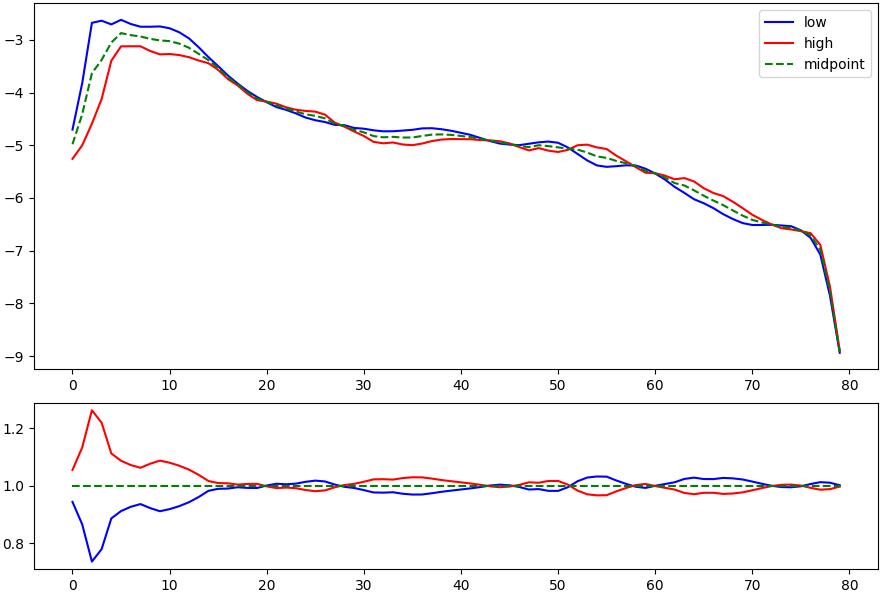
\includegraphics[alt={Compared mel-cepstra of samples rated low vs. high in pitch},width=0.9\linewidth]{highlow.png}
  \caption{MFCCs for high-pitch vs. low-pitch samples}
  \label{fig:highlow}
\end{figure}

This polarisation seemed promising, since we had anticipated the lower and higher samples having some kind of inversely-proportional relationship with respect to timbre. Applying the difference to the input timbre, however, yielded less-than-ideal results, allowing for smooth speech samples only at the extremes (much lower or much higher pitch). An example of the results yielded from gradual timbral modification can be heard in \texttt{audio/voice1\_polarised.wav} in the associated GitHub repository \cite{github}.

We then decided to further segment the dataset, into four groups according to pitch ratings of 1-2, 2-3, 3-4, and 4-5. We then considered the segment that the input sample would be grouped into, and took its difference from the remaining segments. The input sample we were using for testing fit best into the highest segment, so we tested resynthesis by applying the differences of the lower three segments, indicated in \figref{fig:segments}. This approach yielded significantly better results, and would be the foundation for future work.

\begin{figure}
  \centering
  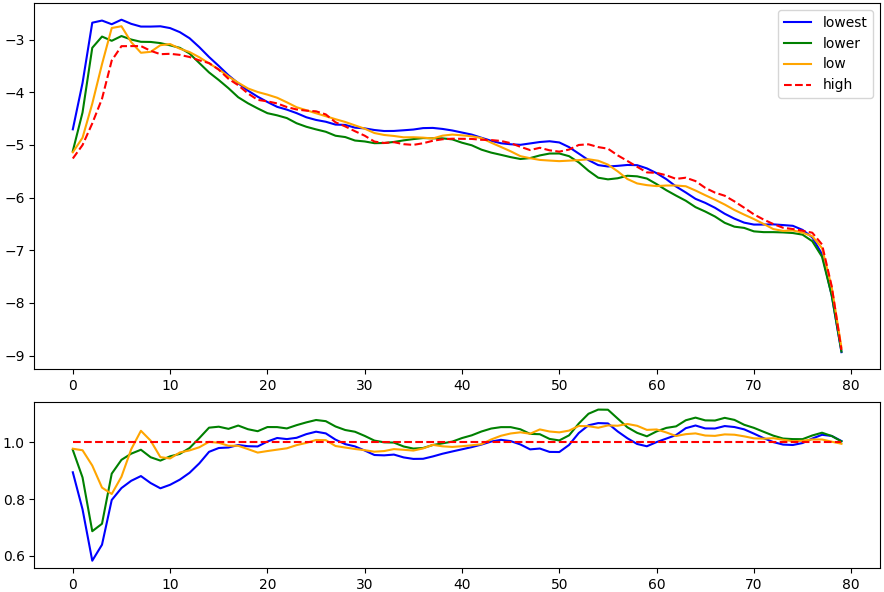
\includegraphics[alt={Compared mel-cepstra of segmented samples},width=0.9\linewidth]{segments.png}
  \caption{MFCCs for segmented samples}
  \label{fig:segments}
\end{figure}


\section{Results}\label{sec:page_size}

Following the segmented dataset approach, smoother results were obtained by editing how exactly the dataset was segmented and the influence the differences between segments had on the input timbre. Particularly, it was found that scaling the difference between the input segment and the others in that dataset drastically improved results, with diminishing returns at around powers of 8. The application of said differences thus followed the format \texttt{input * torch.pow(diff[None,:,None], 8)} where \texttt{input} is the input cepstrogram and \texttt{diff} is the difference between the input segment and another arbitrary segment.

The audio results obtained using a single input file can be heard in the \texttt{audio} directory in \cite{github}. There are 3-4 files per label, alongside an unmodified example. Breathiness and smoothness are two areas of concern: both descriptors lead to a much lower timbre, which is likely due to the distribution of vocal timbres along each rating scale (e.g., lower voices may be more likely to sound rougher) and the distribution of speaker identities in the dataset. The resulting audio files are named according to the timbral descriptor applied, along with a number representing the rating segment used to take the difference. For pitch, the reference segment was 4 except for \texttt{voice1\_Average\_Pitch-4.wav}, which considers segment 3 to be the reference. For example, \texttt{voice1\_Average\_Pitch-3.wav} considered the input file to be in the highest segment (4) and applies the difference calculated from segment 4 to segment 3, resulting in a slightly lower vocal timbre. \texttt{voice1\_Average\_Pitch-1.wav}, on the other hand, uses the difference from segment 4 to segment 1, resulting in a much lower vocal timbre.

This idea of manipulating MFCCs for timbral modification is currently underresearched, since reconstruction of an audio signal was previously impossible without recent developments in machine learning. The results obtained through this project are promising nevertheless, and may pave the way for future research.


\section{Future Work}\label{sec:page_size}
Currently, the reference segment that the input file is grouped into is hard-coded according to the input file being used. By integrating the classifiers discussed, this procedure should be automated to support any operations for any input file.

Additionally, the program expects all samples to have a 16-bit, 24kHz sampling rate, which should also be generalized to support diverse audio files. The program should check the sampling rate of any input file and convert the file manually if the specification is not met.

There may also be room for improvement regarding the generalisation of MFCCs within and between audio samples. The current program sticks to simple averaging, but more sophisticated dimension reduction techniques may improve the accuracy of the generalised cepstra.

We previously proposed the implementation of a user-friendly UI to support the program, but we opted to use our time to dive further into the backend and ensure the results were robust. Future developers may be interested in creating a UI to present the application to users, and consider how users will specify how they want to affect their vocal timbre. An advanced final product may implement a natural language processing model to support textual specification of any number of timbral descriptors. A cheaper alternative may be to resort to a series of sliders corresponding to particular timbre descriptors (e.g., 'breathy', 'nasally', etc.) that reflect exactly the descriptors used during labeling.

Finally, additions to the dataset would improve this project immensely. Given the limited time that we had to do this project, we would want to be able to use a larger dataset for training our model in the future. Ideally, we would like this dataset to be more evenly distributed along different vocal descriptors so when training the model we are able to maintain integrity of other aspects while adjusting one. For example, most raspy voices were lower, therefore the model would make the voice lower while making it more raspy. Also, being able to have an even larger dataset would allow for the model to be able to analyze and understand even more voice types which will help with the quality of outputted voices. As of current, the dataset could only be segmented into four categories for each descriptor due to the relatively low number of samples, but a much larger dataset with a wider variety of vocal timbres would allow for more granular segmentation and thus smaller changes in timbre.


% For BibTeX users:
%\bibliography{ISMIRtemplate}
\begin{thebibliography}{citations}
\bibliographystyle{IEEEtran}
\bibitem{DevExtras}
DevExtras. (2018). Voice Tools. Accessed: Feb. 18, 2025. [Online]. Available: \url{https://devextras.com/voicetools/}

\bibitem{SeekAndNitz}
D. Seek \& C. Nitz (2020). Voice Pitch Analyzer. Accessed: Feb. 18, 2025. [Online]. Available: \url{https://voicepitchanalyzer.app}

\bibitem{AntoniAndSpeechtools}
C. Antoni and C. Speechtools Ltd. (2013). ChristellaVoiceUp. Accessed: Feb. 18, 2025 [Online]. Available: \url{https://www.christellaantoni.co.uk/transgender-voice/voiceupapp/}

\bibitem{Alter24}
I.L. Alter, K.A. Chadwick, K. Andreadis, R. Coleman, M. Pitti, J.M. Ezell, & A. Rameau. “Developing a mobile application for gender‐affirming voice training: A community‐engaged approach“ \textit{Laryngoscope Investig Otolaryngol}. 2024. doi: 10.1002/lio2.70043. Accessed: Feb. 13, 2025. [Online]. Available: \url{https://pmc.ncbi.nlm.nih.gov/articles/PMC11645500}

\bibitem{HawleyAndHancock24}
J.L. Hawley and A.B. Hancock. “Incorporating Mobile App Technology in Voice Modification Protocol for Transgender Women.” Journal of Voice. 2024. DOI: 10.1016/j.jvoice.2021.09.001. Accessed: Feb. 11, 2025. [Online]. Available:
\url{https://www.sciencedirect.com/science/article/abs/pii/S089219972100299X}

\bibitem{Barkmeier-Kraemer}
J.M. Barkmeier-Kraemer, J.N. Craig, A.B. Harmon, R.R. Hillman, J. Jacobson, R.R. Patel, B.H. Ruddy, J.C. Stemple, Y.A. Sumida, K. Tanner, S.M Theis, M.R. van Mersbergen, \& L.P. Verdun. “Voice Disorders.” asha.org. Accessed: Feb. 12, 2025. [Online]. Available: \url{https://www.asha.org/practice-portal/clinical-topics/voice-disorders}

\bibitem{Li22}
J. Li, W. Tu, and L. Xiao. “FreeVC: Towards High-Quality Text-Free One-Shot Voice Conversion,” \textit{arXiv preprint arXiv:2210.15418}, 2022.

\bibitem{PyTorch}
PyTorch, "pytorch," github.com. Acessed Mar. 18, 2025. [Online]. Available: \url{https://github.com/pytorch/pytorch}

\bibitem{Librosa}
Librosa, "librosa," github.com. Acessed Mar. 18, 2025. [Online]. Available: \url{https://github.com/librosa/librosa}

\bibitem{WavLM}
S Chen, C Wang, Z Chen, et al., “Wavlm: Large-scale self-supervised pre-training for full stack speech processing,” \textit{IEEE Journal of Selected Topics in Signal Processing}, 2022.

\bibitem{Nordstrom08}
K. I. Nordstrom, G. Tzanetakis, and P. F. Driessen, "Transforming Perceived Vocal Effort and Breathiness
Using Adaptive Pre-Emphasis Linear Prediction," \textit{IEEE TRANSACTIONS ON AUDIO, SPEECH, AND LANGUAGE PROCESSING}, vol. 16, no. 6, 2008.

\bibitem{SasahireAndHashimoto95}
Y. Sasahira and S. Hashimoto. “Voice Pitch Changing by Linear Predictive Coding Method to Keep the Singer’s Personal Timbre.” \textit{International Computer Music Conference}, (September 3-7) 1995. Available: \url{https://quod.lib.umich.edu/cgi/p/pod/dod-idx/voice-pitch-changing.pdf?c=icmc;idno=bbp2372.1995.118;format=pdf}

\bibitem{Ittichaichareon12}
C. Ittichaichareon, S. Suksri, and T. Yingthawornsuk. "Speech Recognition Using MFCC." \textit{International Conference on Computer Graphics, Simulation and Modeling}, (July 28-29) 2012. Available: \url{https://www.researchgate.net/publication/281446199_Speech_Recognition_using_MFCC}

\bibitem{Lalithaa15}
S. Lalithaa, D. Geyasrutia, R. Narayanana, \& M. Shravani. "Emotion Detection using MFCC and Cepstrum Features." \textit{International Conference on Eco-friendly Computing and Communication Systems}. (2015) Available: \url{https://www.sciencedirect.com/science/article/pii/S1877050915031841?ref=cra_js_challenge&fr=RR-1}

\bibitem{Kong20}
J Kong, J Kim, et al., “Hifi-gan: Generative adversarial networks for efficient and high fidelity speech synthesis," \textit{arXiv preprint arXiv:2010.05646}, 2020.

\bibitem{Mozilla}
Mozilla, 2019, "Common Voice Corpus 1", Common Voice. [Online]. Available: \url{https://commonvoice.mozilla.org/en/datasets}

\bibitem{Pandas}
Pandas, "pandas," github.com. Accessed April 11, 2025. [Online]. Available: \url{https://github.com/pandas-dev/pandas}

\bibitem{Sklearn}
Scikit-learn, "sckit-learn," github.com. Accessed April 7, 2025. [Online]. Available: \url{https://github.com/scikit-learn/scikit-learn}

\bibitem{github}
I. Doyle, A. Klassen, and E. Larmer, "timb-re-synthesis," github.com. Acessed Apr. 16, 2025. [Online]. Available: \url{https://github.com/isaiahdoyle/timb-re-synthesis}

\end{thebibliography}
% For non BibTeX users:
%\begin{thebibliography}{citations}
% \bibitem{Author:17}
% E.~Author and B.~Authour, ``The title of the conference paper,'' in {\em Proc.
% of the Int. Society for Music Information Retrieval Conf.}, (Suzhou, China),
% pp.~111--117, 2017.
%
% \bibitem{Someone:10}
% A.~Someone, B.~Someone, and C.~Someone, ``The title of the journal paper,''
%  {\em Journal of New Music Research}, vol.~A, pp.~111--222, September 2010.
%
% \bibitem{Person:20}
% O.~Person, {\em Title of the Book}.
% \newblock Montr\'{e}al, Canada: McGill-Queen's University Press, 2021.
%
% \bibitem{Person:09}
% F.~Person and S.~Person, ``Title of a chapter this book,'' in {\em A Book
% Containing Delightful Chapters} (A.~G. Editor, ed.), pp.~58--102, Tokyo,
% Japan: The Publisher, 2009.
%
%\end{thebibliography}

\end{document}
